\section{Periodic table}

\begin{figure}[H]
  \centering
  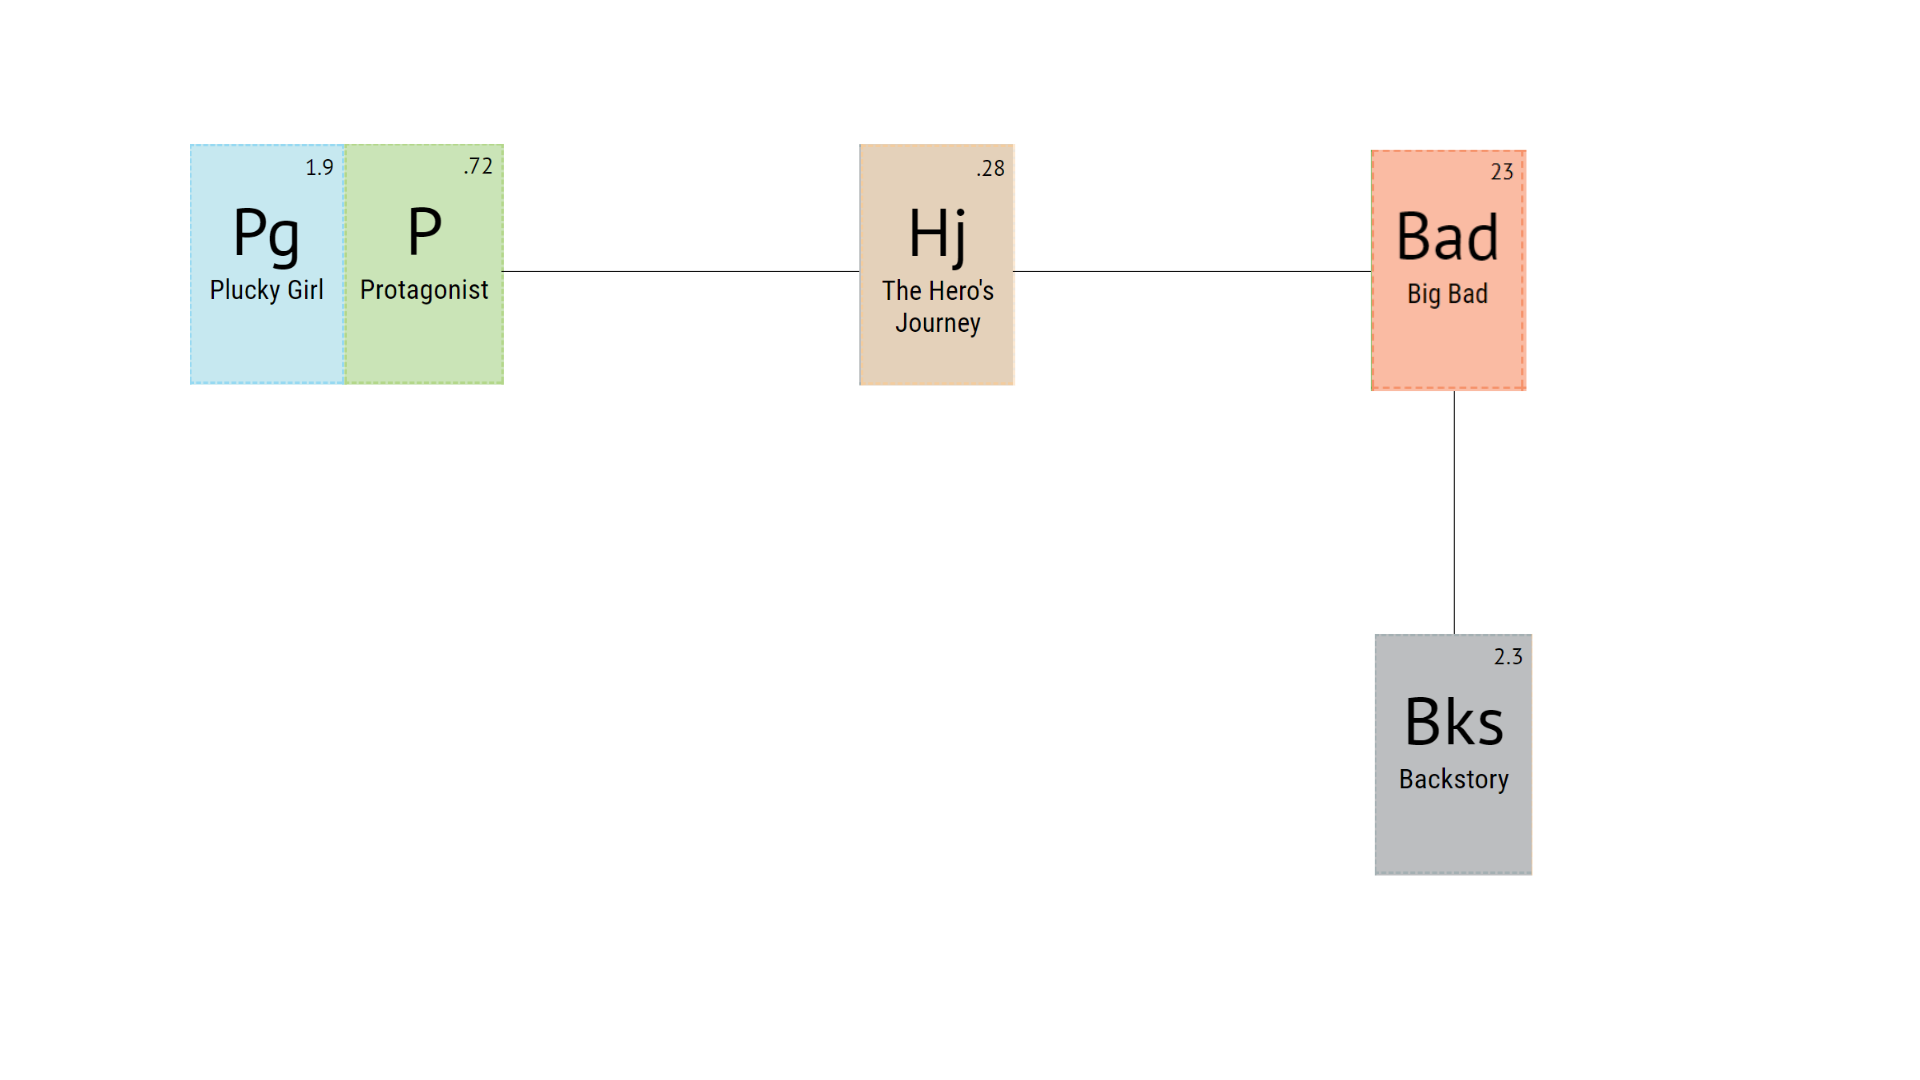
\includegraphics[width=\textwidth]{Images/Diagrams/periodicTable}
  \caption{Tropes form the periodic table of storytelling. Here you can find the full periodic table: \url{http://jamesharris.design/periodic/}}
\end{figure}

\begin{itemize}
\item Pg-P: the protagonist is a brave and optimistic girl. In the course of the story, she will demonstrate her tenacity and her abilities in order to save her beloved. Here are the links to the James Harris' periodic table: \url{https://tvtropes.org/pmwiki/pmwiki.php/Main/PluckyGirl} - \url{https://tvtropes.org/pmwiki/pmwiki.php/Main/TheProtagonist}

\item Hj: the story is based on the Hero's Journey pattern described by Joseph Campbell. The journey of the protagonist come with a call to adventure (her beloved is missing) and will finish with a homecoming. Here is the link to the James Harris' periodic table: \url{https://tvtropes.org/pmwiki/pmwiki.php/Main/TheHerosJourney}

\item Bad: the main antagonist is the cause of all bad happenings in the story.Here is the link to the James Harris' periodic table: \url{https://tvtropes.org/pmwiki/pmwiki.php/Main/BigBad}

\item Bks: the background story explains the fundamental reason why the main antagonist has turned evil.Here is the link to the James Harris' periodic table: \url{https://tvtropes.org/pmwiki/pmwiki.php/Main/Backstory}
\end{itemize}
